\question
Конструктор занимается проектированием игрового робота, который должен уметь передвигаться по плоскости и стрелять. Для этого роботу требуется двигатель, который обеспечивает движение, и механизм стрельбы. Каждый из этих механизмов можно установить на отдельные валы, но инженеры стремятся минимизировать количество валов для экономии места внутри робота. Некоторые механизмы, например, лазерный прицел и механизм захвата предметов, не должны находиться на одном валу из-за электромагнитных вмешательств.

Дана таблица с парами таких механизмов. Крестиками обозначены механизмы, которые не могут находиться на одном валу. Найдите минимальное число валов, на которые можно поместить механизмы робота, соблюдая все ограничения.

\begin{minipage}[h]{0.45\linewidth}
\center{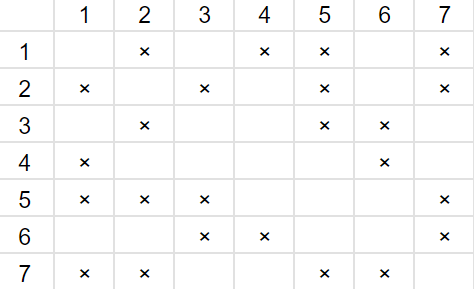
\includegraphics[width=0.7\textwidth]{pic/122.png} }
\end{minipage}

Внимание! Если ваша картинка не прогрузилась, загляните в папку "недостающие картинки" на гугл-диске с типовиком.

---------------

Автор -- Александр Лазарев